\label{cap:metodologia}

In questo capitolo viene descritto l'approccio metodologico adottato per lo sviluppo del framework di rilevamento delle vulnerabilità. L'obiettivo è superare le limitazioni intrinseche dei modelli LLM generalisti attraverso due approcci distinti:

\begin{itemize}
    \item Il \textbf{Fine-Tuning supervisionato} (orientato al ragionamento \textit{Chain-of-Thought}), impiegato per adattare i modelli al dominio specifico di Algorand (PyTeal).
    \item Il \textbf{Retrieval-Augmented Generation (RAG)}, che interviene durante l'inferenza per ancorare l'analisi a dati fattuali. Il RAG opera fornendo al modello descrizioni dettagliate e istruzioni sulle vulnerabilità pertinenti al codice in esame, arricchendo il prompt con snippet di codice vulnerabile simile e sfruttando così il potente paradigma dell'\textit{In-Context Learning} (\textit{Few-Shot Learning}).
\end{itemize}

La Figura \ref{fig:rag_architecture} illustra il flusso logico della pipeline di audit proposta. Il sistema si configura come un'architettura \textit{LLM-Centric} in cui il modello interviene attivamente nelle due fasi critiche del processo (evidenziate dai blocchi tratteggiati a sinistra):

\begin{enumerate}
    \item \textbf{Fase di Retrieval:} In cui il modello è chiamato a generare descrizioni semantiche del codice target, necessarie per interrogare in modo efficace il database vettoriale.
    \item \textbf{Fase di Audit:} In cui il modello analizza il codice target, contestualizzato e arricchito dagli esempi recuperati dal RAG, per identificare le vulnerabilità.
\end{enumerate}

L'intero processo di \textit{Fine-Tuning}, discusso in dettaglio nel corso del capitolo, è stato calibrato specificamente per far sì che i modelli base interiorizzino questi task. In questo modo, il modello fine-tuned è non solo in grado di astrarre correttamente il codice nella fase di Retrieval, ma risulta anche predisposto a recepire e applicare in modo ottimale il contesto fornito \textit{on-the-fly} nella fase di Audit.

Al fine di garantire la totale trasparenza e riproducibilità degli esperimenti condotti in questo lavoro di tesi, l'intero codice sorgente, i dataset generati e i prompt utilizzati per l'addestramento e la valutazione dei modelli sono stati resi open-source\footnote{Il materiale completo relativo a questo lavoro di tesi è pubblicamente accessibile sulla repository GitHub: \url{https://github.com/NickTor99/llm_based_vulnerability_detection_algorand.git}}.


\newpage

\begin{figure}[ht!]
    \centering
    \begin{tikzpicture}[
        node distance=2.0cm,
        auto,
        % Stile blocchi processo principale
        block/.style={
            rectangle, 
            draw, 
            fill=blue!10, 
            text width=4.5cm, 
            text centered, 
            rounded corners, 
            minimum height=1.2cm,
            font=\small
        },
        % Stile input/output
        cloud/.style={
            draw, 
            ellipse, 
            fill=green!10, 
            minimum height=1cm,
            text width=2.5cm,
            text centered,
            font=\footnotesize
        },
        % Stile storage (Vector DB)
        storage/.style={
            cylinder, 
            draw, 
            shape border rotate=90, 
            aspect=0.25, 
            fill=orange!10, 
            text width=2.5cm, 
            text centered, 
            minimum height=2.0cm, 
            font=\small
        },
        % NUOVO STILE: Chiamata al Modello LLM
        llm/.style={
            rectangle,
            draw=purple!80!black,
            fill=purple!10,
            thick,
            dashed,
            text width=3cm,
            text centered,
            minimum height=1cm,
            font=\footnotesize\bfseries
        },
        line/.style={draw, -latex, thick},
        description/.style={fill=white, inner sep=2pt, font=\scriptsize, align=center}
    ]

    % --- COLONNA CENTRALE (Pipeline) ---
    \node [cloud] (input) {Input \\ Contratto PyTeal};
    
    % Step 1: Generazione Descrizione
    \node [block, below of=input, node distance=2.5cm] (desc_gen) {Generazione \\ Descrizione Semantica};
    
    % Step 2: Embedding
    \node [block, below of=desc_gen, node distance=2.0cm] (embed) {Embedding Query \\ ($v_{query}$)};
    
    % Step 3: Ricerca
    \node [block, below of=embed, node distance=2.0cm] (search) {Cosine Similarity \\ Search};
    
    % Step 4: Assemblaggio Prompt
    \node [block, below of=search, node distance=2.5cm] (prompt) {Assemblaggio \\ Prompt Dinamico}; 
    
    % Step 5: Audit Finale
    \node [block, below of=prompt, node distance=2.0cm] (audit_step) {Analisi e Audit \\ Vulnerabilità};

    \node [cloud, below of=audit_step, node distance=2.0cm] (output) {Report Output};

    % --- COLONNA DESTRA (Storage) ---
    % Vector Store posizionato lateralmente rispetto alla ricerca
    \node [storage, right of=search, node distance=6cm] (vectorstore) {\textbf{Vector Knowledge Base}};

    % --- COLONNA SINISTRA (LLM Calls) ---
    % Chiamata LLM per la Descrizione (Task 3)
    \node [llm, left of=desc_gen, node distance=5.5cm] (llm_desc) {LLM Call};
    
    % Chiamata LLM per l'Audit (Task 1/2)
    \node [llm, left of=audit_step, node distance=5.5cm] (llm_audit) {LLM Call};

    % --- ARROWS (Connessioni) ---
    
    % Flusso Verticale
    \path [line] (input) -- (desc_gen);
    \path [line] (desc_gen) -- (embed);
    \path [line] (embed) -- (search);
    \path [line] (search) -- node[description, pos=0.5] {Top-k Indices} (prompt);
    \path [line] (prompt) -- (audit_step);
    \path [line] (audit_step) -- (output);

    % Connessioni LLM (Bidirezionali logiche o indicazione di processo)
    \draw [line, dashed, <->] (desc_gen) -- node[above, font=\scriptsize] {Inference} (llm_desc);
    \draw [line, dashed, <->] (audit_step) -- node[above, font=\scriptsize] {Inference} (llm_audit);

    % Connessioni Vector Store
    \draw [line] (search) -- node[description, below] {Query} (vectorstore);
    \draw [line] (vectorstore) |- node[description, near end] {Retrieval Context \\ (Snippet + Vuln Info)} (prompt);

    \end{tikzpicture}
    \caption{Architettura della pipeline RAG.}
    \label{fig:rag_architecture}
\end{figure}

\section{Analisi Preliminare e Definizione della Knowledge Base}
\label{sec:analisi_preliminare}

La fase cruciale che precede l'implementazione tecnica è la costruzione di una documentazione dettagliata e strutturata sulle vulnerabilità oggetto di studio. Questa "base di conoscenza" non funge solo da riferimento teorico, ma costituisce il pilastro fondamentale per due processi chiave:
\begin{enumerate}
    \item \textbf{Generazione del Dataset CoT:} Per addestrare il modello a "ragionare", è necessario fornirgli spiegazioni logiche che colleghino il codice PyTeal alla specifica vulnerabilità.
    \item \textbf{Popolamento del Vector Database:} La documentazione viene indicizzata nel sistema RAG per essere recuperata in tempo reale come contesto durante l'analisi.
\end{enumerate}

\subsection{Struttura del Profilo di Vulnerabilità}
Per ogni vulnerabilità selezionata, basandoci sulla mappatura OWASP per Algorand \cite{boi2025}, è stato creato un profilo tecnico standardizzato composto da quattro elementi essenziali:

\begin{itemize}
    \item \textbf{Descrizione Tecnica:} Definizione della vulnerabilità nel contesto dell'Algorand Virtual Machine (AVM).
    \item \textbf{Vettori di Attacco (Trigger):} Identificazione dei pattern di codice o delle condizioni transazionali che permettono l'exploit.
    \item \textbf{Security Checks:} I controlli logici e le pre-condizioni che l'auditor (o il modello) deve verificare nel codice.
    \item \textbf{Strategie di Mitigazione:} Tecniche di codifica sicura (es. asserzioni su \texttt{Txn.rekey\_to()} o \texttt{Txn.sender()}) necessarie per prevenire il problema.
\end{itemize}

\subsection{Dettaglio delle Classi di Vulnerabilità Analizzate}
Le informazioni tecniche relative alle vulnerabilità sono state estratte e rielaborate a partire dalla documentazione di sicurezza di settore fornita da Trail of Bits \cite{trailofbits_algorand}, integrata con la mappatura tassonomica OWASP proposta in letteratura \cite{boi2025}.

\subsubsection{Access Control (V1)}
Queste vulnerabilità riguardano la gestione non autorizzata delle applicazioni e dei flussi di fondi.

\paragraph{Arbitrary Update e Delete} 
Si presentano nelle \textit{Stateful Applications} quando le funzioni amministrative non sono protette.
\begin{itemize}
    \item \textbf{Descrizione Tecnica:} Il contratto espone le operazioni \texttt{UpdateApplication} o \texttt{DeleteApplication} senza verificare l'identità del chiamante, permettendo la modifica della logica o la distruzione dell'istanza.
    \item \textbf{Vettori di Attacco:} Un attaccante invia una transazione con \texttt{OnComplete} impostato su \textit{Update} o \textit{Delete}, sostituendo il programma con codice malevolo o eliminando lo stato globale.
    \item \textbf{Security Checks:} Verificare la presenza di branch condizionali che gestiscono \texttt{OnComplete.UpdateApplication} e \texttt{DeleteApplication}.
    \item \textbf{Strategie di Mitigazione:} Inserire un controllo esplicito che imponga \texttt{Txn.sender() == Global.creator\_address()} prima di approvare queste operazioni.
\end{itemize}

\paragraph{Unchecked Payment e Asset Receiver}
Riguardano la mancata validazione del destinatario in transazioni di trasferimento fondi.
\begin{itemize}
    \item \textbf{Descrizione Tecnica:} Il contratto autorizza transazioni di tipo \texttt{Pay} o \texttt{Axfer} (Asset Transfer) senza validare i campi \texttt{Receiver} o \texttt{AssetReceiver}.
    \item \textbf{Vettori di Attacco:} Un attaccante invia (o inietta in un gruppo) una transazione in cui il campo ricevente è impostato sul proprio indirizzo, dirottando i fondi del contratto.
    \item \textbf{Security Checks:} Analizzare tutte le inner transaction o le validazioni di gruppo per confermare che i campi \textit{Receiver} siano confrontati con valori attesi.
    \item \textbf{Strategie di Mitigazione:} Implementazione di whitelist rigorose (es. \texttt{Txn.receiver() == Addr(...)}) o hardcoding degli indirizzi autorizzati nel contratto.
\end{itemize}

\subsubsection{Unchecked External Calls: Rekeying e Chiusura Account (V6)}
Questa categoria rappresenta il rischio di cessione del controllo dell'account o drenaggio totale degli asset.

\paragraph{Unchecked Rekey To}
Rappresenta uno dei rischi più critici specifici dell'AVM, legato al cambio dell'autorità di firma.
\begin{itemize}
    \item \textbf{Descrizione Tecnica:} La vulnerabilità si verifica quando una transazione approvata da una \textit{LogicSig} non verifica che il campo \texttt{rekey\_to} sia vuoto.
    \item \textbf{Vettori di Attacco:} Un attaccante invia una transazione di pagamento o trasferimento asset impostando \texttt{rekey\_to} sul proprio indirizzo, ottenendo il controllo totale dell'account vittima.
    \item \textbf{Security Checks:} Verificare che ogni transazione (eccetto \texttt{ApplCall}) includa il controllo sul campo di rekeying.
    \item \textbf{Strategie di Mitigazione:} Imporre assertivamente che \texttt{Txn.rekey\_to() == Global.zero\_address()} in tutti i rami logici del contratto.
\end{itemize}

\paragraph{Unchecked Close Remainder To e Asset Close To}
Riguardano i meccanismi di chiusura dei conti e il trasferimento del saldo residuo.
\begin{itemize}
    \item \textbf{Descrizione Tecnica:} I campi \texttt{CloseRemainderTo} (per ALGO) e \texttt{AssetCloseTo} (per ASA) permettono di chiudere un account inviando tutto il saldo rimanente a un indirizzo target.
    \item \textbf{Vettori di Attacco:} Un attaccante costruisce una transazione che imposta se stesso come destinatario della chiusura (\textit{close-out target}), drenando interamente i fondi.
    \item \textbf{Security Checks:} Scansionare il codice per assicurarsi che questi campi siano esplicitamente controllati e non lasciati al valore di default (che potrebbe essere manipolato).
    \item \textbf{Strategie di Mitigazione:} Validare che tali campi siano sempre \texttt{Global.zero\_address()}, a meno che la chiusura non sia una funzionalità intenzionale verso un indirizzo fidato predefinito.
\end{itemize}

\subsubsection{Denial of Service: Unchecked Transaction Fee (V10)}
Sfrutta le dinamiche economiche e il meccanismo di \textit{fee pooling} di Algorand.

\begin{itemize}
    \item \textbf{Descrizione Tecnica:} Il contratto approva transazioni senza imporre un limite superiore al campo \texttt{fee}, esponendosi ad abusi economici.
    \item \textbf{Vettori di Attacco:} Un attaccante invia una transazione con una fee eccessiva (es. 1000 ALGO invece di 0.001), svuotando il saldo del contratto o dell'account pagante tramite \textit{fee pooling}.
    \item \textbf{Security Checks:} Verificare la presenza di controlli di disuguaglianza sul campo \texttt{Txn.fee()}.
    \item \textbf{Strategie di Mitigazione:} Definire una costante \texttt{MAX\_FEE} (es. 2000 microAlgo) e imporre \texttt{Txn.fee() <= Int(MAX\_FEE)}.
\end{itemize}

\section{Creazione del Dataset}
\label{sec:dataset_creation}

La qualità della rilevazione delle vulnerabilità dipende direttamente dalla ricchezza e dalla varietà del dataset utilizzato per il fine-tuning. Per questo lavoro, è stato costruito un dataset specializzato di smart contract in PyTeal, progettato per addestrare il modello non solo a identificare una vulnerabilità, ma a seguire un percorso logico rigoroso per giustificarne la presenza.

\subsection{Raccolta dei Dati e Fonti}
Il processo di raccolta ha portato alla selezione di un corpus totale di 110 smart contract per le fasi di addestramento e validazione (100 per il training e 10 per la validazione). La fonte primaria è stata il repository ufficiale di Algorand dedicato a PyTeal \cite{algorand_pyteal_github}, dal quale sono stati estratti template di logiche reali e ampiamente utilizzate, tra cui:
\begin{itemize}
    \item Protocolli di Finanza Decentralizzata (DeFi) e \textit{Automated Market Makers} (AMM).
    \item Servizi di \textit{Escrow} e \textit{Atomic Swaps}.
    \item Sistemi di pagamento ricorrenti gestiti tramite \textit{Smart Signatures}.
    \item Contratti di \textit{Crowdfunding} e sistemi di \textit{Governance/Voting}.
\end{itemize}

Per garantire che il modello imparasse a distinguere tra implementazioni sicure e vulnerabili all'interno dello stesso contesto logico, si è proceduto con l'iniezione manuale delle vulnerabilità. Partendo dai contratti sicuri recuperati, sono state introdotte varianti malevole modificando o eliminando i controlli di sicurezza critici definiti nella Sezione \ref{sec:analisi_preliminare}. Questo approccio permette di avere coppie di contratti con logica di business quasi identica ma con profili di sicurezza opposti, costringendo il modello a focalizzarsi sui dettagli semantici del codice piuttosto che sulla struttura generale.

\subsection{Composizione del Dataset}
Il dataset di addestramento (100 campioni) è stato bilanciato per coprire uniformemente tutte le classi di vulnerabilità analizzate:
\begin{itemize}
    \item \textbf{80\% Campioni Vulnerabili:} Suddivisi equamente (10\% per ogni categoria) tra le 8 vulnerabilità in esame (Arbitrary Update/Delete, Unchecked RekeyTo, ecc.).
    \item \textbf{20\% Campioni Sicuri:} Contratti privi di vulnerabilità o con mitigazioni correttamente implementate.
\end{itemize}

In casi di scarsità di esempi reali per specifiche combinazioni di opcode, si è fatto ricorso alla generazione di \textit{synthetic data}, ricreando snippet di codice minimi ma sintatticamente corretti che isolassero il pattern vulnerabile. Per la fase di valutazione finale delle performance, è stato preparato un set di test indipendente composto da \textbf{45 smart contracts}, distribuito in 5 campioni per ogni tipologia di vulnerabilità e 5 campioni sicuri.

\subsection{Modellazione del Dataset e Tassonomia dei Task}
\label{sec:training_tasks}

A partire dal corpus iniziale di 100 smart contract, il dataset di fine-tuning è stato costruito adottando un approccio di \textit{Instruction Tuning}. Ogni contratto non è stato inserito nel dataset come semplice testo grezzo, ma è stato trasformato in molteplici esempi di addestramento strutturati come coppie \texttt{(Prompt, Risposta Ideale)}.

Per garantire che il modello apprendesse non solo a "leggere" il codice, ma a comportarsi secondo pattern operativi specifici, sono stati definiti tre task distinti. Questa strategia di \textit{Multi-Task Learning} ha permesso di generare, per ogni singolo contratto, diverse istanze di training che forzano il modello ad adattare la propria risposta (il \textit{Target Output}) a seconda dell'obiettivo dell'audit.

\subsubsection{Task 1: Vulnerability Detection}
Questo task costituisce il nucleo dell'addestramento alla sicurezza. Qui la risposta del training set è stata progettata per insegnare al modello il processo deduttivo completo.
\begin{itemize}
    \item \textbf{Struttura del Prompt:} Include il codice completo e un'istruzione generica ("Esegui un audit di sicurezza di questo contratto").
    \item \textbf{Ingegneria della Risposta (Target):} La risposta fornita nel dataset non è un semplice verdetto. È stata costruita includendo obbligatoriamente il tag \texttt{<think>} contenente un'analisi step-by-step del flusso di esecuzione, seguito dal tag \texttt{<final>} con il report delle vulnerabilità trovate.
    \item \textbf{Obiettivo:} Addestrare il modello a non saltare alle conclusioni, ma a generare esplicitamente la catena di pensiero (\textit{Chain-of-Thought}) prima di emettere un giudizio.
\end{itemize}

\subsubsection{Task 2: Targeted Vulnerability Verification}
In questo scenario, gli esempi di training sono stati modellati per simulare un'interazione guidata, preparatoria all'integrazione con il sistema RAG.
\begin{itemize}
    \item \textbf{Struttura del Prompt:} L'istruzione non è generica, ma contiene un'ipotesi specifica da verificare (es. "Analizza se il contratto è vulnerabile a \textit{Unchecked RekeyTo}").
    \item \textbf{Ingegneria della Risposta (Target):} La risposta target è focalizzata esclusivamente sulla verifica della vulnerabilità richiesta, ignorando altri potenziali difetti.
    \item \textbf{Utilità:} Questo insegna al modello a operare come un "verificatore di ipotesi". In fase di inferenza (come descritto nei capitoli successivi), quando il RAG inietterà un sospetto di vulnerabilità nel prompt, il modello saprà attivare questo specifico pattern di attenzione focalizzata per confermare o smentire il suggerimento.
\end{itemize}

\subsubsection{Task 3: Semantic Code Description}
Per questo task le risposte riguardano la comprensione funzionale profonda del codice.
\begin{itemize}
    \item \textbf{Struttura del Prompt:} Richiede di descrivere la logica di business del contratto (es. "Descrivi lo scopo, l'architettura e le funzionalità di questo codice PyTeal").
    \item \textbf{Struttura della Risposta (Target):} La risposta ideale è formattata come un riassunto tecnico strutturato a punti elenco, che deve obbligatoriamente evidenziare tre livelli di caratteristiche semantiche:
    \begin{enumerate}
        \item \textbf{Tipologia Architetturale:} Classificazione del contratto come \textit{Stateful Application} (gestione di stato globale/locale) o \textit{Stateless LogicSig} (firma delegata), fondamentale per capire il contesto di esecuzione.
        \item \textbf{Intento Funzionale:} Definizione dello scopo ad alto livello (es. "Escrow Account", "Voting System", "NFT Marketplace").
        \item \textbf{Logica di Validazione:} Analisi dettagliata dei controlli implementati sui campi delle transazioni (es. verifica su \texttt{Txn.fee}, \texttt{Txn.rekey\_to}) e restrizioni sull'uso di specifici OpCode critici (es. presenza di \texttt{InnerTxnBuilder}).
    \end{enumerate}
    \item \textbf{Obiettivo:} Questo task ha una duplice valenza:
    \begin{enumerate}
        \item \textbf{Istruisce il modello a comprendere la sinstassi del linguaggio.}
        \item \textbf{Standardizza l'output per la creazione degli embeddings.} Le descrizioni generate secondo questo schema fisso saranno utilizzate per popolare il Database Vettoriale, permettendo il recupero di contratti "simili" basato sulla logica (semantica) e non solo sulla sovrapposizione di parole chiave (sintassi).
    \end{enumerate}
\end{itemize}

\subsection{Sviluppo del Dataset Chain-of-Thought (CoT)}
\label{sec:cot_methodology}

Una delle innovazioni centrali di questo lavoro risiede nell'abbandono del paradigma di classificazione binaria "codice-etichetta" in favore della tecnica \textit{Chain-of-Thought} (CoT). Mentre l'addestramento tradizionale spinge il modello a eseguire un semplice \textit{pattern matching} — ovvero l'identificazione di una vulnerabilità basata sulla frequenza statistica di certi termini nel training set — la CoT forza il modello a simulare un processo di \textit{System 2 reasoning} \cite{wei2022chain}.

\subsubsection{Vantaggi del Ragionamento Sequenziale nell'Audit}
L'utilizzo della CoT è supportato dalla letteratura recente, la quale dimostra che i modelli di linguaggio, se istruiti a "mostrare il proprio lavoro" tramite passaggi intermedi, migliorano drasticamente le prestazioni in compiti di ragionamento logico e simbolico \cite{wei2022chain}. Nel contesto degli smart contract Algorand, questo approccio è fondamentale per due ragioni:
\begin{itemize}
    \item \textbf{Decomposizione del Problema:} Il modello impara a scomporre l'analisi in blocchi logici (Handler di creazione, gestione dei NoOp, controlli amministrativi), emulando il comportamento di un auditor umano.
    \item \textbf{Riduzione delle Allucinazioni:} Obbligando il modello a identificare esplicitamente le pre-condizioni (es. "il contratto è una Smart Signature?") e a verificare i campi transazionali prima di dare una risposta, si riduce il rischio che il modello dichiari una vulnerabilità basandosi su euristiche errate.
\end{itemize}

\subsubsection{Ingegneria delle Risposte di Training}
Le risposte fornite nel dataset di addestramento sono state costruite seguendo una struttura rigorosa divisa in due fasi: l'audit di sicurezza (Thinking) e il verdetto finale (Evaluation).

\subsubsection{Fase di Security Audit (Tag \texttt{<think>})}
In questa sezione, il modello esegue una scansione riga per riga o blocco per blocco del contratto PyTeal. Il ragionamento non si limita a cercare errori, ma convalida anche le parti sicure, costruendo un contesto di analisi completo. Come evidenziato in studi precedenti, la capacità di ragionare su pattern linguistici interpretabili permette agli LLM di fornire spiegazioni in linguaggio naturale che aumentano la fiducia nell'output del sistema \cite{wei2022chain}.

\subsubsection{Verdetto Finale (Tag \texttt{<final>})}
Al termine del processo di analisi, il modello sintetizza i risultati in una valutazione finale che include:
\begin{itemize}
    \item \textbf{Vulnerability Name:} Il nome tecnico della falla riscontrata (es. \textit{Unchecked Asset Receiver}).
    \item \textbf{Motivation:} Una sintesi logica del motivo per cui quel frammento di codice è insicuro.
    \item \textbf{Risk Level:} Una valutazione della gravità dell'impatto (Critical, High, Medium, Low).
\end{itemize}

\subsubsection{Esempio di Struttura CoT nel Dataset}
Per illustrare la metodologia, si riporta di seguito un esempio di istanza di addestramento relativa a una vulnerabilità di tipo \textit{Unchecked Asset Receiver}.

\begin{lstlisting}[caption={Esempio di ragionamento CoT per l'analisi di un contratto PyTeal}, label={lst:cot_example}]
### Thinking:
L'analisi sistematica del contratto rivela una struttura di trasferimento asset gestita tramite l'handler NoOp. 
1. Handler di Creazione: Corretto, assegna correttamente il mittente come creatore.
2. Handler Update/Delete: Implementano controlli di accesso rigorosi (creator-only).
3. NoOp Handler (Analisi Critica): Il contratto convalida gli argomenti e la presenza dell'asset, ma utilizza `Txn.accounts[1]` direttamente come destinatario del trasferimento.
4. Identificazione del Rischio: Poiche l'array `accounts` e fornito dall'utente e non e validato dal contratto, qualsiasi chiamante puo dirottare i fondi verso un indirizzo arbitrario.

<|end thinking|>

### Final Evaluation: Il contratto contiene una vulnerabilita critica nel NoOp handler: l'indirizzo del ricevente dell'asset non viene validato, permettendo il drenaggio dei fondi.
### Vulnerability: Unchecked Asset Receiver
### Risk: Critical - Perdita totale degli asset detenuti dal contratto.
\end{lstlisting}

\subsection{Efficienza dei Dati e Limitazioni Dimensionali}
\label{sec:dataset_limitations}

Un aspetto critico di questa ricerca riguarda la scala dimensionale del dataset utilizzato. A fronte di approcci tradizionali di Deep Learning che fanno affidamento su decine di migliaia di esempi, il corpus curato per questo lavoro conta circa\textbf{ 500 istanze di instruction tuning}(derivate dai 100 smart contract base).
Questa scelta, sebbene imposta in parte dalla scarsità di risorse pubbliche, trova una giustificazione teorica e pratica nella natura stessa del task di ragionamento.

\subsubsection{Il Paradigma "Quality over Quantity"}
La letteratura recente sull'allineamento dei modelli (es. il paper LIMA - \textit{Less Is More for Alignment}) \cite{zhou2023lima} suggerisce che, per insegnare a un modello "come" eseguire un task complesso (Instruction Tuning), la qualità e la densità informativa degli esempi sono nettamente più determinanti della loro quantità.
Nel nostro caso, ogni esempio del dataset non è una semplice coppia (Input, Label), ma include una \textit{Chain-of-Thought} densa e dettagliata. Il modello, quindi, non deve apprendere statisticamente la distribuzione dei token di tutti i possibili contratti PyTeal (task che richiederebbe milioni di esempi), ma deve apprendere il \textbf{pattern di ragionamento} per l'audit. Un numero ridotto di esempi, se estremamente curati e diversificati nella logica, è sufficiente per trasferire questa competenza metodologica.

\subsubsection{Vincoli del Dominio e Limitazioni}
È doveroso riconoscere che la dimensione contenuta del dataset (100 contratti unici di base) rappresenta una limitazione oggettiva:
\begin{itemize}
    \item \textbf{Scarsità di Dati:} A differenza dell'ecosistema Ethereum/Solidity, per il quale esistono dataset pubblici massivi, l'ecosistema PyTeal manca di repository standardizzati di vulnerabilità. La costruzione manuale del dataset è stata un passaggio obbligato che ha limitato la scalabilità numerica.
    \item \textbf{Rischio di Overfitting e Copertura:} Esiste il rischio concreto che il modello possa sovra-adattarsi alle specifiche strutture sintattiche presenti nel training set, faticando a generalizzare su stili di coding radicalmente diversi o su tipologie di contratti non rappresentate (es. logiche di governance molto complesse non incluse nei 100 contratti base).
\end{itemize}

\subsubsection{Validità Metodologica Nonostante i Limiti}
Nonostante tali limitazioni, la metodologia proposta mantiene la sua validità scientifica e i risultati (discussi nel Capitolo 4) risultano robusti grazie all'architettura ibrida adottata:
\begin{enumerate}
    \item \textbf{Generalizzazione del Processo, non dei Dati:} L'obiettivo del Fine-Tuning CoT non è insegnare al modello a memorizzare i bug, ma a seguire una procedura di controllo. Una volta appreso che "bisogna controllare il campo \texttt{rekey\_to}", il modello tende ad applicare questa logica anche a contratti mai visti, mitigando l'effetto del dataset piccolo.
    \item \textbf{Ruolo Compensativo del RAG:} La vera mitigazione alla limitata "conoscenza parametrica" derivante dai pochi esempi è il sistema RAG. Anche se il modello non ha mai visto un certo tipo di contratto nel training, il RAG recupera frammenti simili o regole di sicurezza pertinenti al momento dell'inferenza, fornendo il contesto mancante.
\end{enumerate}

In conclusione, mentre un dataset più ampio rimarrebbe desiderabile per coprire l'intera varianza semantica possibile, l'approccio \textit{High-Quality CoT + RAG} potrebbe dimostrarsi una strategia efficace per massimizzare le prestazioni in scenari con scarsità di dati come quello della sicurezza su Algorand.

\section{Selezione dei Modelli e Parametri di Scaling}
\label{sec:model_selection}

La scelta dell'architettura e della dimensione del modello (parameter count) rappresenta una decisione progettuale critica. Per questo lavoro, la selezione è ricaduta su modelli di taglia "medium-large" (nello specifico la classe dei 32B), escludendo i modelli "small" (<15B) e ponendo i modelli "large" (>70B) come oggetto di sviluppi futuri.

\subsection{Giustificazione Teorica: La Curva a U del Reasoning}
Questa decisione metodologica trova fondamento nelle recenti scoperte riguardanti le leggi di scaling per il ragionamento logico. Secondo Wang et al. (2025) \cite{wang2025larger}, la capacità di un modello di inferire regole logiche complesse non segue una crescita lineare semplice rispetto alla dimensione, ma è caratterizzata da una curva a U determinata dalla complessità del compito.

I punti chiave derivanti da questa teoria che hanno guidato la selezione sono:
\begin{itemize}
    \item \textbf{Optimal Model Size e Entropia:} Esiste una dimensione ottimale del modello che permette di massimizzare il ragionamento riducendo l'overfitting. Il paper dimostra che l'entropia di ricerca del problema (Graph Search Entropy) è linearmente correlata alla dimensione del modello necessaria \cite{wang2025larger}. 
    \item \textbf{Soglia di Complessità:} L'audit di smart contract PyTeal richiede l'analisi di dipendenze multi-hop e stati globali, configurandosi come un compito ad alta entropia. Modelli sottodimensionati non possiedono la densità parametrica sufficiente per mappare queste regole latenti, limitandosi a un riconoscimento sintattico superficiale.
\end{itemize}

\subsection{Studio Pilota e Definizione della Soglia Minima}
In fase preliminare, è stato condotto un test qualitativo per confrontare la capacità di analisi di modelli di diverse classi di grandezza (14B vs 32B). 
Coerentemente con la teoria, i modelli da 14B, pur mostrando competenza sintattica, hanno fallito nel mantenere la coerenza nella fase di \textit{Chain-of-Thought}, spesso interrompendo la catena logica necessaria per individuare vulnerabilità semantiche complesse. Al contrario, i modelli della classe 32B (Qwen3-32B e QwQ-32B) hanno dimostrato la stabilità necessaria per completare il percorso di audit.

\subsection{Limiti Computazionali e Sviluppi Futuri}
Sebbene la teoria suggerisca che modelli di dimensioni ancora maggiori (es. Llama-3 70B o Qwen-72B) potrebbero offrire margini ulteriori di miglioramento sulla parte ascendente della curva di reasoning, la presente ricerca si è limitata alla soglia dei 32B.
Tale scelta rappresenta un trade-off necessario dettato dai vincoli di risorse computazionali (VRAM e potenza di calcolo) disponibili per la fase di fine-tuning. L'esplorazione del comportamento asintotico della curva di performance su modelli \textit{large-scale}, al fine di verificare se l'incremento di parametri porti a rendimenti decrescenti o a nuove capacità emergenti nel contesto specifico di Algorand, è lasciata come direzione per lavori futuri.

\subsection{La Scelta della Famiglia Qwen: Qwen3 e QwQ}
\label{sec:qwen_selection}

All'interno della classe dimensionale dei 32 miliardi di parametri, la selezione dell'architettura specifica è ricaduta sulla famiglia di modelli \textbf{Qwen3} e, in particolare, sulla variante \textbf{QwQ} (Qwen with Questions/Reasoning). Questa decisione è motivata da caratteristiche architetturali che li pongono allo stato dell'arte (SOTA) per i compiti di \textit{Code Intelligence} e ragionamento logico.

\subsubsection{Ottimizzazione Nativa per il "Thinking"}
A differenza dei modelli generalisti tradizionali, progettati per fornire risposte dirette, la variante \textbf{QwQ} è stata addestrata specificamente per emulare processi di ragionamento. \cite{wang2025larger}. Questo significa che il modello è intrinsecamente predisposto a generare tracce di pensiero intermedie prima di formulare una conclusione.
Questa caratteristica si allinea perfettamente con la metodologia \textit{Chain-of-Thought} (CoT) adottata in questa tesi (descritta nella Sezione \ref{sec:dataset_creation}):
\begin{itemize}
    \item \textbf{Allineamento col Dataset:} Poiché il nostro dataset di fine-tuning utilizza i tag \texttt{<think>} e \texttt{<final>}, l'utilizzo di un modello base già ottimizzato per separare il ragionamento dalla risposta riduce drasticamente il tempo di convergenza durante il training.
    \item \textbf{Deep Reasoning:} QwQ ha dimostrato capacità superiori nel gestire problemi matematici e logici complessi, una competenza trasferibile all'analisi dei flussi di esecuzione degli smart contract PyTeal, dove è necessario tracciare variabili attraverso molteplici step transazionali.
\end{itemize}

\subsubsection{Performance SOTA nella categoria 32B}
Analisi comparative indipendenti e benchmark di settore (es. HumanEval, MBPP) evidenziano come la famiglia Qwen3-32B superi regolarmente i concorrenti diretti (come Llama-3 di pari taglia) in task di programmazione e comprensione del codice.
La combinazione di una forte base di conoscenza sul codice (Qwen3) e di una specializzazione nel ragionamento step-by-step (QwQ) fornisce il substrato ideale per massimizzare l'efficacia del Fine-Tuning e del RAG, permettendo al sistema di "navigare" la complessità delle vulnerabilità Algorand con un'accuratezza che modelli non specializzati nel reasoning faticano a raggiungere.

\section{Configurazione Finetuning}

\label{sec:training_setup}

L'addestramento di modelli di grandi dimensioni (32 miliardi di parametri) presenta sfide significative in termini di memoria VRAM e tempi di calcolo. Per mitigare questi vincoli senza compromettere le prestazioni, il processo di fine-tuning è stato implementato utilizzando il framework \textbf{Unsloth}, una libreria che ottimizza i kernel di backpropagation e la gestione della memoria.

\subsection{Quantizzazione e Low-Rank Adaptation (QLoRA)}
Il modello base \texttt{Qwen3-32B(o (QwQ-32B))} è stato caricato utilizzando la tecnica di quantizzazione a 4-bit (NF4 - NormalFloat 4-bit), che riduce drasticamente l'impronta di memoria mantenendo una precisione paragonabile ai 16-bit. 
Per l'adattamento dei pesi, si è adottata la metodologia QLoRA applicata a tutti i moduli lineari del modello (inclusi \texttt{q\_proj}, \texttt{k\_proj}, \texttt{v\_proj}, \texttt{gate\_proj}, \texttt{up\_proj}, \texttt{down\_proj}). Questa scelta è cruciale: a differenza dei primi approcci LoRA che targettizzavano solo i moduli di attenzione, estendere l'adattamento ai moduli MLP (Feed-Forward Networks) migliora significativamente le capacità di ragionamento del modello.

I parametri specifici di LoRA sono stati configurati con un rango $r=64$ e un fattore di scaling $\alpha=128$. Un rango elevato ($r=64$ rispetto allo standard $r=8$ o $r=16$) è stato scelto per garantire che il modello avesse sufficiente capacità espressiva per apprendere le complesse regole semantiche del linguaggio PyTeal e le strutture di ragionamento Chain-of-Thought.

\subsection{Iperparametri di Addestramento}
Il training è stato eseguito in modalità \textit{Supervised Fine-Tuning} (SFT) per 3 epoche totali, ritenute sufficienti per la convergenza su un dataset di dimensioni contenute (~500 esempi) evitando fenomeni di overfitting. 
Per ottimizzare l'uso della memoria, è stata utilizzata una dimensione del batch per device pari a 1, compensata da un accumulo dei gradienti (\textit{Gradient Accumulation}) di 8 step, risultando in una \textit{effective batch size} di 8.

L'ottimizzatore scelto è \texttt{paged\_adamw\_8bit}, che gestisce in modo efficiente i picchi di memoria trasferendo gli stati dell'ottimizzatore dalla GPU alla CPU quando necessario. La strategia di learning rate prevede un \textit{warmup} iniziale del 5\% dei passi totali seguito da un decadimento con profilo coseno (\textit{Cosine Decay}), partendo da un learning rate massimo di $5e^{-5}$.

\begin{table}[!h]
    \centering
    \renewcommand{\arraystretch}{1.2}
    \begin{tabular}{|l|l|}
        \hline
        \textbf{Parametro} & \textbf{Valore / Configurazione} \\
        \hline
        \hline
        \multicolumn{2}{|c|}{\textit{Modello e Adattamento}} \\
        \hline
        Modello Base & Unsloth/Qwen3-32B(QwQ-32B) \\
        Quantizzazione & 4-bit (NF4) \\
        Metodo PEFT & LoRA (QLoRA) \\
        LoRA Rank ($r$) & 64 \\
        LoRA Alpha ($\alpha$) & 128 \\
        Target Modules & All Linear Layers (Attention + MLP) \\
        Dropout & 0.0 \\
        \hline
        \multicolumn{2}{|c|}{\textit{Training Dynamics}} \\
        \hline
        Epoche & 3 \\
        Effective Batch Size & 8 (1 per device $\times$ 8 accumulation) \\
        Learning Rate & $5 \times 10^{-5}$ \\
        Scheduler & Cosine (Warmup ratio: 0.05) \\
        Optimizer & Paged AdamW 8-bit \\
        Max Sequence Length & 2048 tokens \\
        Weight Decay & 0.02 \\
        Gradient Checkpointing & Attivo (Unsloth optimized) \\
        Seed & 3407 \\
        \hline
        
    \end{tabular}
    \caption{Iperparametri e Configurazione del Fine-Tuning}
    \label{fig:hyperparameters}
\end{table}

La Tabella \ref{fig:hyperparameters} riassume la configurazione completa utilizzata per gli esperimenti.

\subsection{Prompt Template e Strategia di Loss}
\label{sec:chat_template_loss}

Oltre alla configurazione degli iperparametri, un aspetto cruciale per il successo del fine-tuning di modelli orientati al ragionamento (Reasoning Models) è la corretta formattazione dei token di input e la focalizzazione del segnale di apprendimento.

\subsubsection{Personalizzazione del Chat Template (Jinja2)}
I modelli della famiglia Qwen utilizzano nativamente il formato ChatML. Tuttavia, per supportare la metodologia \textit{Chain-of-Thought} e la struttura multi-task definita nella Sezione \ref{sec:training_tasks}, è stato necessario iniettare un chat template personalizzato (implementato in Jinja2) direttamente nel tokenizer.

Il template progettato svolge tre funzioni critiche:
\begin{enumerate}
    \item \textbf{Enforcement Strutturale:} Definisce rigidamente i confini tra i ruoli (\texttt{system}, \texttt{user}, \texttt{assistant}) utilizzando i token speciali \texttt{<|im\_start|>} e \texttt{<|im\_end|>}.
    \item \textbf{Segregazione del Ragionamento:} Introduce tag XML-like specifici (\texttt{<think>} e \texttt{<final>}) per separare il flusso di pensiero latente dalla risposta finale. Questo forza il modello a generare prima il blocco di ragionamento (audit step-by-step) e solo successivamente il verdetto, impedendo risposte impulsive.
    \item \textbf{Gestione Dinamica dei Task:} Il template contiene una logica condizionale che adatta l'output in base al tipo di task. Se il messaggio contiene un campo \texttt{thinking}, il template apre il blocco di pensiero; se contiene solo una \texttt{description} (per il Task 3 di descrizione semantica), genera direttamente il contenuto finale.
\end{enumerate}

Questa strutturazione garantisce che, durante l'inferenza, il modello non si limiti a predire il token successivo in base alla probabilità statistica generica, ma segua uno schema cognitivo preordinato.

\subsubsection{Ottimizzazione della Loss: Training on Responses Only}
Per massimizzare l'efficienza dell'addestramento, si è adottata la strategia di \textit{Response Masking}, configurata tramite la direttiva \texttt{train\_on\_responses\_only}.
In un processo di fine-tuning standard, la funzione di perdita (Cross-Entropy Loss) viene calcolata su tutti i token della sequenza, inclusi quelli del prompt utente. Tuttavia, nel nostro scenario, non è desiderabile che il modello "impari" a riprodurre i prompt o il codice PyTeal fornito in input (che sono fissi), ma solo l'analisi prodotta in output.

Utilizzando i delimitatori \\\\ \texttt{instruction\_part="<|im\_start|>user"} e \texttt{response\_part="<|im\_end|>user"} \\\\ il trainer è stato configurato per mascherare (ignorare) i token relativi all'istruzione durante il calcolo dei gradienti. I vantaggi di questo approccio sono duplici:
\begin{itemize}
    \item \textbf{Focalizzazione del Gradiente:} Il modello aggiorna i propri pesi basandosi esclusivamente sull'errore commesso nel generare il ragionamento (\texttt{<think>}) e la valutazione finale (\texttt{<final>}). Questo accelera la convergenza verso il comportamento desiderato.
    \item \textbf{Prevenzione dell'Overfitting:} Si evita che il modello memorizzi pattern irrilevanti presenti nei prompt di istruzione, riducendo il rischio di bias verso specifici formati di input.
\end{itemize}

\subsection{Analisi delle Curve di Apprendimento e Prevenzione dell'Overfitting}
\label{sec:loss_analysis}

Per validare la stabilità del processo di fine-tuning e determinare il punto di arresto ottimale (\textit{Early Stopping}), sono state monitorate le curve di Training Loss e Validation Loss per entrambi i modelli addestrati (Qwen3-32B e QwQ-32B). I dati sono stati raccolti a intervalli regolari di 10 step.

\subsubsection{Visualizzazione delle Performance}
La Figura \ref{fig:loss_curves} illustra l'andamento delle loss durante i 180 step di addestramento (corrispondenti a 3 epoche).

\begin{figure}[ht]
    \centering
    \begin{subfigure}[b]{0.48\textwidth}
        \centering
        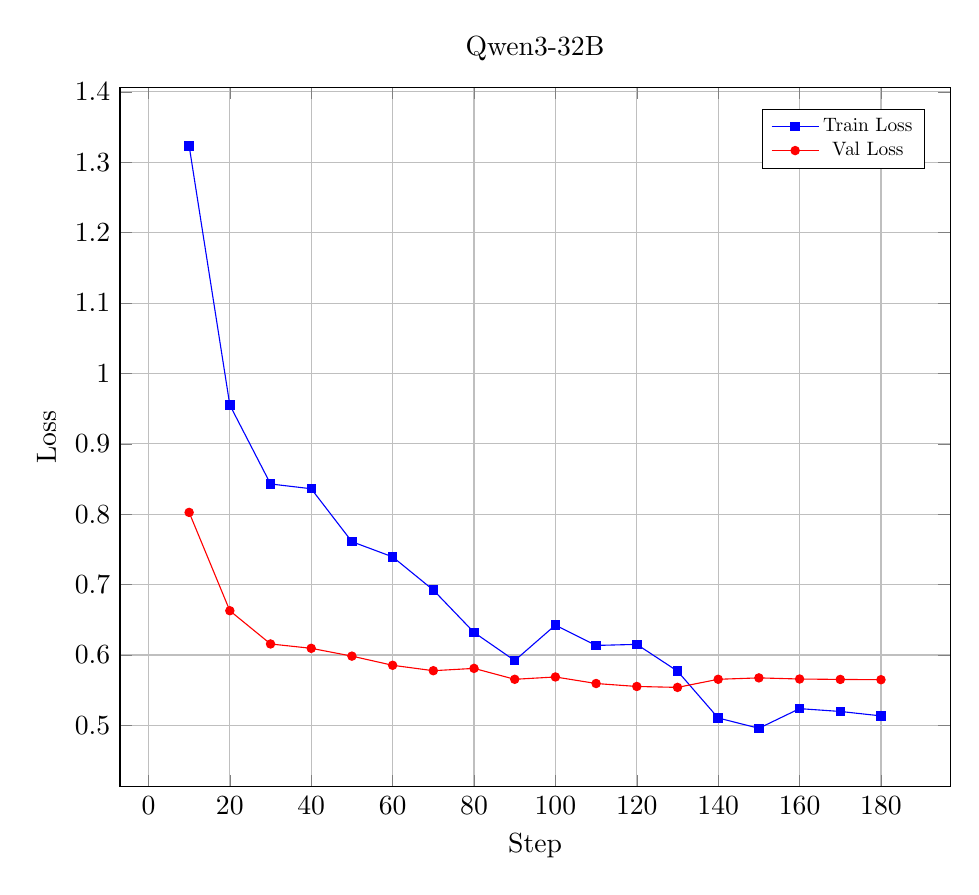
\begin{tikzpicture}
            \begin{axis}[
                title={Qwen3-32B},
                xlabel={Step},
                ylabel={Loss},
                grid=major,
                width=\textwidth,
                legend pos=north east,
                legend style={nodes={scale=0.7, transform shape}} 
            ]
            \addplot[color=blue,mark=square*,mark size=1.5pt] coordinates {
                (10,1.3234) (20,0.9551) (30,0.8430) (40,0.8362) (50,0.7610)
                (60,0.7394) (70,0.6923) (80,0.6321) (90,0.5921) (100,0.6425)
                (110,0.6136) (120,0.6151) (130,0.5771) (140,0.5105) (150,0.4959)
                (160,0.5238) (170,0.5198) (180,0.5135)
            };
            \addlegendentry{Train Loss}
            
            \addplot[color=red,mark=*,mark size=1.5pt] coordinates {
                (10,0.8026) (20,0.6629) (30,0.6157) (40,0.6095) (50,0.5984)
                (60,0.5854) (70,0.5777) (80,0.5810) (90,0.5655) (100,0.5688)
                (110,0.5595) (120,0.5553) (130,0.5540) (140,0.5655) (150,0.5675)
                (160,0.5659) (170,0.5653) (180,0.5649)
            };
            \addlegendentry{Val Loss}
            \end{axis}
        \end{tikzpicture}
        \caption{Curve di Loss per Qwen3-32B}
    \end{subfigure}
    \hfill
    \begin{subfigure}[b]{0.48\textwidth}
        \centering
        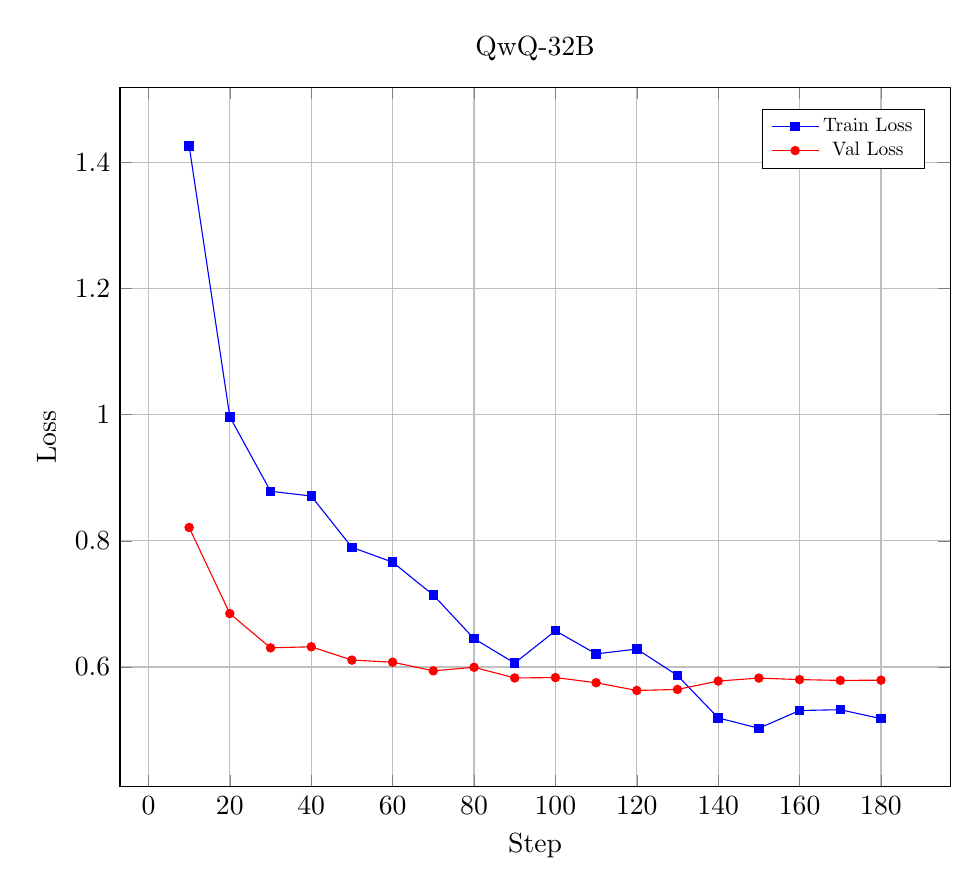
\begin{tikzpicture}
            \begin{axis}[
                title={QwQ-32B},
                xlabel={Step},
                ylabel={Loss},
                grid=major,
                width=\textwidth,
                legend pos=north east,
                legend style={nodes={scale=0.7, transform shape}}
            ]
            \addplot[color=blue,mark=square*,mark size=1.5pt] coordinates {
                (10,1.4258) (20,0.9963) (30,0.8785) (40,0.8709) (50,0.7896)
                (60,0.7662) (70,0.7140) (80,0.6450) (90,0.6062) (100,0.6575)
                (110,0.6208) (120,0.6285) (130,0.5866) (140,0.5194) (150,0.5030)
                (160,0.5311) (170,0.5324) (180,0.5182)
            };
            \addlegendentry{Train Loss}
            
            \addplot[color=red,mark=*,mark size=1.5pt] coordinates {
                (10,0.8211) (20,0.6847) (30,0.6304) (40,0.6321) (50,0.6110)
                (60,0.6077) (70,0.5940) (80,0.5996) (90,0.5827) (100,0.5833)
                (110,0.5751) (120,0.5629) (130,0.5645) (140,0.5778) (150,0.5825)
                (160,0.5801) (170,0.5788) (180,0.5792)
            };
            \addlegendentry{Val Loss}
            \end{axis}
        \end{tikzpicture}
        \caption{Curve di Loss per QwQ-32B}
    \end{subfigure}
    \caption{Confronto delle dinamiche di apprendimento. Si nota come la Validation Loss raggiunga un minimo intorno allo step 120-130 per poi stabilizzarsi o risalire, indicando il punto ottimale di arresto.}
    \label{fig:loss_curves}
\end{figure}

\subsubsection{Interpretazione e Strategia Anti-Overfitting}
L'analisi dei grafici evidenzia un comportamento coerente con la teoria dell'apprendimento profondo su dataset di dimensioni limitate. 
\begin{itemize}
    \item \textbf{Fase di Convergenza Rapida (Step 0-100)}: Entrambi i modelli mostrano una discesa ripida della Training Loss nei primi 100 step (da $\sim1.4$ a $\sim0.6$). Questo indica che i modelli stanno apprendendo efficacemente la sintassi del Chain-of-Thought e la struttura del linguaggio PyTeal. La Validation Loss segue lo stesso trend, confermando che l'apprendimento è generalizzabile.
    \item \textbf{Il Punto di Inflessione e l'Overfitting (Step 120-180)}: Intorno allo step 120-130 si osserva un fenomeno critico, particolarmente evidente nel modello QwQ-32B:
\begin{itemize}
    \item La \textbf{Training Loss} continua a scendere costantemente (raggiungendo 0.51), indicando che il modello sta iniziando a memorizzare i dettagli specifici degli esempi di training.
    \item La \textbf{Validation Loss}, al contrario, smette di migliorare. Per Qwen3 raggiunge un plateau ($\sim0.555$), mentre per QwQ inizia una leggera risalita (da $0.562$ a $0.582$).
\end{itemize}

Questo pattern, noto come \textit{Generalization Gap}, segnala l'inizio dell'overfitting. Se l'addestramento fosse proseguito oltre le 3 epoche (180 step), il modello avrebbe massimizzato la performance sui dati visti a discapito della capacità di analizzare nuovi contratti, memorizzando le vulnerabilità invece di apprenderne la logica.
\end{itemize}

\subsubsection{Decisione sulla Durata del Training}
Sulla base di questi dati empirici, la scelta di limitare il training a \textbf{3 epoche} si è rivelata ottimale. Questa configurazione permette di fermare il processo esattamente nella "Goldilocks Zone" (zona ideale), dove il modello ha acquisito la capacità di ragionamento (Validation Loss minima) ma non ha ancora iniziato a degradare le sue capacità predittive su dati non visti.
In particolare, per il modello QwQ, che mostra una sensibilità maggiore all'overfitting dovuta verosimilmente alla sua natura specializzata nel reasoning, l'arresto tempestivo è stato determinante per preservarne la robustezza.

\section{Implementazione della Pipeline RAG}
\label{sec:rag_implementation}

L'efficacia della Retrieval Augmented Generation (RAG) dipende strettamente dalla qualità e dall'organizzazione della base di conoscenza sottostante. In questa fase, è stato costruito un \textit{Vector Store} specializzato, progettato per fornire al modello non solo definizioni teoriche, ma esempi pratici di codice vulnerabile semanticamente affini al contratto in analisi.

\subsection{Costruzione del Database Vettoriale e Indicizzazione}
Per l'archiviazione e il recupero efficiente delle informazioni, si è optato per un'implementazione di \textit{Local Vector Store} persistente. Questa scelta architetturale permette di gestire gli embeddings e i metadati associati in un formato serializzato a bassa latenza, eliminando l'overhead di gestione di un servizio database distribuito per un corpus di dimensioni contenute.

\subsubsection{Composizione del Corpus di Riferimento}
La Knowledge Base del RAG è stata popolata selezionando un sottoinsieme curato di \textbf{40 smart contract vulnerabili}, bilanciati equamente per coprire le 8 classi di vulnerabilità analizzate (5 esempi rappresentativi per ogni tipologia, come \textit{Unchecked RekeyTo}, \textit{Arbitrary Update}, ecc.).

Ogni voce indicizzata nel Vector Store non è costituita dall'intero codice sorgente grezzo, ma è strutturata come un oggetto composito contenente tre campi informativi chiave:

\begin{enumerate}
    \item \textbf{Vulnerability Label (Metadato):} Un riferimento tassonomico alla specifica vulnerabilità presente. Questo campo funge da chiave esterna per collegare lo snippet alle definizioni teoriche e alle regole di mitigazione descritte nella Sezione \ref{sec:analisi_preliminare}.
    
    \item \textbf{Semantic Description (Vettore di Ricerca):} 
    Questo è il campo principale utilizzato per il calcolo della similarità. Invece di indicizzare il codice PyTeal (che può variare sintatticamente), è stata indicizzata una descrizione in linguaggio naturale della logica del contratto.
    
    \item \textbf{Vulnerable Snippet (Payload):} Il frammento di codice isolato che contiene l'errore logico. Questo payload non viene vettorializzato, ma viene recuperato e iniettato nel prompt come esempio \textit{Few-Shot} ("Ecco come appare questa vulnerabilità in un codice simile") per guidare l'attenzione del modello.
\end{enumerate}

\subsubsection{Processo di Embedding}
Le descrizioni semantiche sono state trasformate in rappresentazioni vettoriali dense utilizzando un modello di embedding pre-addestrato (es. \texttt{hkunlp/instructor-xl}), generando vettori a $N$ dimensioni ottimizzati per catturare le sfumature della logica di business degli smart contract.


\subsection{Workflow Operativo della Pipeline RAG}
\label{sec:retrieval_workflow}

Il processo di interrogazione del sistema RAG non avviene tramite una semplice ricerca per parole chiave, ma segue una pipeline multistadio progettata per massimizzare la rilevanza semantica e la diversità degli esempi forniti. La Figura \ref{fig:rag_architecture} illustra il flusso logico completo, dall'input del codice alla generazione del prompt ingegnerizzato. La procedura si articola in quattro fasi sequenziali:

\subsubsection{Fase 1: Generazione della descrizione}
Per avviare il processo di retrieval, il sistema interroga inizialmente l'LLM sotto esame, richiedendo la generazione della Code Description del contratto target. Questa operazione converte il codice grezzo in una descrizione in linguaggio naturale, che verrà utilizzata come query normalizzata per l'interrogazione del database vettoriale.
\textbf{Nota sulla Coerenza Semantica:} È imperativo che il prompt utilizzato in questa fase di inferenza contenga le medesime istruzioni impiegate durante la costruzione del Vector Store. Mantenere una rigorosa omogeneità strutturale tra la descrizione generata real-time (Query) e quelle indicizzate nella Knowledge Base è condizione necessaria per evitare disallineamenti nello spazio vettoriale e garantire l'ottimalità del retrieval.

\subsubsection{Fase 2: Embedding e Ranking per Similarità}
La descrizione generata viene convertita in un vettore denso ($v_{query}$) utilizzando il medesimo modello di embedding impiegato per l'indicizzazione.
Il sistema esegue quindi una ricerca di similarità coseno ($Sim(v_{query}, v_{doc})$) all'interno del Local Vector Store. Il risultato è una lista preliminare di candidati ordinati in modo decrescente in base al punteggio di similarità, che rappresenta quanto la logica del contratto in esame è vicina a quella dei contratti vulnerabili noti.

\subsubsection{Fase 3: Selezione e Diversificazione dei Risultati}
Per massimizzare l'efficacia del contesto senza introdurre informazioni ridondanti (come fornire al modello molteplici esempi della stessa identica tipologia di errore), il sistema applica un criterio di diversificazione.

L'algoritmo non si limita a prendere i risultati con il punteggio più alto in assoluto, ma seleziona i migliori $N$ contratti che appartengono a \textbf{classi di vulnerabilità differenti}. Il processo segue una logica di filtraggio sequenziale:
\begin{enumerate}
    \item Viene sempre selezionato il contratto con la similarità semantica più alta (il "best match").
    \item Scorrendo i risultati successivi, vengono scartati quelli che presentano una vulnerabilità già inclusa nella selezione corrente.
    \item L'iterazione prosegue fino al raggiungimento di $N$ esempi distinti (nel nostro caso sperimentale, $N=3$).
\end{enumerate}
Questo approccio garantisce che il prompt finale offra al modello una panoramica variegata dei potenziali rischi, coprendo diverse tipologie di minacce pertinenti alla logica analizzata.

\subsubsection{Fase 4: Context Injection e Prompting Few-Shot}
Nella fase conclusiva, il sistema estrae dal Vector Store il payload informativo associato agli $N$ candidati selezionati. Questo payload, composto dallo \textbf{snippet di codice vulnerabile} e dalla relativa \textbf{descrizione tecnica} della vulnerabilità, viene iniettato nel System Prompt.
L'assemblaggio finale segue il paradigma \textit{Few-Shot Learning}: il modello riceve esempi concreti di "come appare un errore simile" nel codice che sta analizzando, guidando l'attenzione verso pattern specifici senza dover fare affidamento esclusivamente sulla propria memoria parametrica.

\subsection{Costruzione Dinamica del Prompt}
\label{sec:prompt_engineering}

Una volta recuperati i contratti simili dalla Knowledge Base, la fase finale consiste nell'assemblare il prompt da inviare al modello. Per garantire un audit completo e sistematico, è stata introdotta una \textbf{Checklist Dinamica}: una lista di controllo che guida il modello passo dopo passo, indicando quali controlli effettuare e con quale priorità.

\subsubsection{Ordinamento e Priorità dei Controlli}
Invece di chiedere genericamente di "trovare errori", il prompt fornisce al modello l'elenco completo delle 8 classi di vulnerabilità studiate. Tuttavia, l'ordine di questa lista non è fisso, ma cambia per ogni contratto analizzato in base ai risultati del RAG:

\begin{enumerate}
    \item \textbf{Alta Priorità (Top-N):} Le vulnerabilità associate ai contratti più simili recuperati (i primi $N$) vengono posizionate in cima alla lista. Accanto ad esse viene mostrato il punteggio di similarità (es. 0.92), segnalando al modello che è molto probabile riscontrare quel problema specifico e di verificarlo per primo.
    \item \textbf{Copertura Totale:} Le restanti vulnerabilità, anche se hanno ottenuto un punteggio di similarità basso, non vengono eliminate ma posizionate in fondo alla lista. Questo serve per sicurezza: anche se il sistema RAG non ha trovato corrispondenze forti, il modello deve comunque effettuare un controllo di base per tutte le possibili minacce, evitando di ignorare a priori delle categorie.
\end{enumerate}

\subsubsection{Gestione del Contesto e Dettagli}
La scelta di inserire i dettagli completi (lo snippet di codice vulnerabile e la descrizione estesa) solo per i primi $N$ contratti simili risponde a un preciso bilanciamento:
\begin{itemize}
    \item \textbf{Evitare Confusione:} Inserire troppi esempi nel prompt (ad esempio 10 snippet diversi) rischierebbe di confondere il modello, rendendo difficile distinguere tra il codice da analizzare e gli esempi forniti.
    \item \textbf{Contesto Sufficiente:} Limitarsi ai pochi esempi più rilevanti permette di fornire un aiuto mirato dove serve di più, mantenendo il prompt pulito e focalizzato sul contratto in esame.
\end{itemize}

Per la configurazione sperimentale adottata in questa tesi, basata su modelli della classe \textbf{32 Miliardi di parametri} (Qwen3-32B), il valore è stato fissato a \textbf{$N=3$}. Questa decisione è motivata dai limiti della finestra di contesto efficace: inserire un numero eccessivo di esempi rischierebbe di diluire l'attenzione del modello, riducendo la capacità di focalizzarsi sul codice target.

Tuttavia, l'architettura della pipeline è progettata per essere scalabile. L'utilizzo futuro di modelli con capacità superiori (es. Llama-3 70B o modelli proprietari con context window estese) permetterebbe di incrementare il valore di $N$ ($N > 3$), arricchendo ulteriormente il contesto con una maggiore varietà di scenari di vulnerabilità senza compromettere la stabilità del ragionamento.

\subsubsection{Struttura del Prompt Generato}
Il risultato di questo processo è un prompt strutturato che guida il modello passo-passo. Di seguito si riporta un estratto reale della sezione \textit{Checklist} generata per un contratto di test:

\begin{lstlisting}[caption={Esempio di Checklist Dinamica iniettata nel System Prompt}, label={lst:checklist_prompt}, basicstyle=\ttfamily\footnotesize, frame=single]
-------------------------------- CheckList --------------------------------
1. **Arbitrary delete** (Score: 0.9255)
   - Description: If UpdateApplication calls are not properly restricted 
     to authorized entities, attackers can destroy the contract.
   - Preconditions: Applies to stateful apps handling DeleteApplication.
   - Security Check: Ensure DeleteApplication is restricted to creator/admin.

2. **Arbitrary update** (Score: 0.9101)
   - Description: Unrestricted UpdateApplication allows logic replacement.
   - Preconditions: Handling of OnComplete.UpdateApplication.
   - Security Check: Verify Txn.sender == Global.creator_address.

3. **Unchecked Asset Receiver** (Score: 0.9079)
   - Description: Missing validation on AssetReceiver allows theft.
   - Preconditions: TxnType.AssetTransfer transactions.
   - Security Check: Ensure asset transfer goes to whitelisted addresses.

4. **Unchecked Payment Receiver** (Score: 0.9049)
   [...Dettagli condensati...]

5. **Unchecked Close Remainder To** (Score: 0.8967)
   [...Dettagli condensati...]

[...]

8. **Unchecked Rekey to** (Score: 0.8916)
   [...Dettagli condensati...]
---------------------------------------------------------------------------
ISTRUZIONI PER L'AUDIT:
Usa la lista sopra come guida prioritaria. Analizza il codice passo dopo passo
nel blocco <think>, verificando le precondizioni per ogni punto della lista.
\end{lstlisting}

Questa presentazione impone al modello (specialmente grazie al fine-tuning CoT) di scorrere mentalmente la lista dall'item 1 all'item 8, dedicando maggiore attenzione computazionale (più token di \textit{thinking}) agli elementi ad alto score, senza però ignorare totalmente il resto dello spettro di sicurezza.

\section{Ottimizzazione del Retrieval}
\label{sec:retrieval_optimization}

Una criticità intrinseca della soluzione RAG proposta risiede nel disallineamento tra la similarità semantica (funzionale) e la similarità di sicurezza. È pertanto essenziale adottare strategie mirate affinché il sistema di retrieval recuperi esempi rilevanti per la specifica vulnerabilità, e non meramente per la logica applicativa.
L'utilizzo di una descrizione generica del codice tenderebbe, infatti, a raggruppare gli Smart Contract nello spazio vettoriale in base al loro contenuto semantico predominante: tutti i contratti di tipo \textit{Asta} risulterebbero vicini tra loro, così come quelli di \textit{Voting} o \textit{Token Swap}.
Tuttavia, tale prossimità vettoriale può essere ingannevole: due contratti funzionalmente identici (es. due aste) possono presentare profili di sicurezza opposti, dove il primo implementa correttamente i controlli sulle fee, mentre il secondo ne è privo.

\subsection{Security Code Description}
\label{sec:sec_code_desc}
Per mitigare il bias funzionale, la nostra pipeline evita l'indicizzazione del codice grezzo, adottando invece una rappresentazione intermedia generata tramite LLM.
Abbiamo implementato una fase di pre-processing, che prevede la generazione di descrizioni in linguaggio naturale guidate da prompt specifici.

Il prompt di indicizzazione istruisce il modello a operare secondo due direttive principali:
\begin{itemize}
    \item \textbf{Astrazione Sintattica:} Il modello è istruito a omettere rigorosamente i nomi specifici delle variabili, i valori hardcoded e i commenti originali presenti nel codice sorgente. Questi elementi introducono "rumore" nello spazio vettoriale, allontanando contratti che implementano la stessa logica di sicurezza ma con stili di coding diversi.
    \item \textbf{Mappatura dei Controlli di Sicurezza:} La descrizione generata deve concentrarsi esclusivamente sulle logiche di validazione, evidenziando in modo esplicito quali campi sensibili delle transazioni risultano verificati e, soprattutto, quali campi critici rimangono non controllati (es. "Manca il controllo esplicito sul campo \texttt{RekeyTo} nella transazione di pagamento").
\end{itemize}

In questo modo, l'embedding viene calcolato su una sintesi che mappa la "struttura della vulnerabilità" piuttosto che la mera "funzione del contratto". Ciò incrementa drasticamente la probabilità che, analizzando un target vulnerabile, il sistema recuperi un esempio affetto dalla medesima falla di sicurezza.

In questo contesto, l'obiettivo del RAG non è fornire un termine di paragone generico, bensì rispondere puntualmente alla domanda: "Il contratto target presenta pattern sovrapponibili a una vulnerabilità nota?".

\section{Validazione Comparativa: Fine-Tuning vs Modelli SOTA Generalisti}
\label{sec:finetuning_rationale}

A conclusione della definizione metodologica, è doveroso porsi un interrogativo critico sulla validità dell'intero processo di addestramento. Nell'attuale panorama dell'Intelligenza Artificiale, dominato da \textit{Large Language Models} di scala massiva (come GPT-5, Claude 3.5 o DeepSeek-V3), la tendenza prevalente è quella di sfruttare le enormi capacità di generalizzazione di questi sistemi tramite tecniche avanzate di \textit{Prompt Engineering}, evitando i costi e la complessità del fine-tuning.

Pertanto, un'altra domanda di ricerca discussa nella fase sperimentale (Capitolo 5) è la seguente: \textit{Ha ancora senso investire risorse nel fine-tuning di modelli "piccoli" (32B) su domini specifici, o i modelli giganti generalisti rendono questa pratica obsoleta?}

\subsection{Adattamento vs Generalizzazione}
Per rispondere a questa domanda, lo studio non si limita a testare i modelli addestrati, ma include un benchmark comparativo diretto contro modelli allo Stato dell'Arte (SOTA) di dimensioni nettamente superiori (es. DeepSeek-V3, un'architettura MoE da 671B parametri totali), utilizzati in modalità \textit{In-Context Learning} (solo Prompt Engineering).

L'analisi si basa sul confronto tra due vantaggi competitivi opposti:

\begin{itemize}
    \item \textbf{Vantaggio dei Modelli Generalisti (The "Giant" Approach):}
    Grazie alla loro immensa base di conoscenza e al numero di parametri, questi modelli possiedono capacità di ragionamento logico superiori e una vasta cultura generale. Possono adattarsi a nuovi compiti semplicemente tramite istruzioni nel prompt, senza richiedere aggiornamenti dei pesi. Tuttavia, operano come "generalisti": potrebbero conoscere la sintassi di PyTeal, ma mancare delle sfumature specifiche di sicurezza derivanti dall'esperienza pratica su quella specifica blockchain.
    
    \item \textbf{Vantaggio del Fine-Tuning (The "Specialist" Approach):}
    Il modello da 32B, pur avendo una capacità di ragionamento "grezza" inferiore, è stato esposto intensivamente a esempi specifici di audit. L'ipotesi è che la specializzazione possa compensare la minore taglia, permettendo al modello piccolo di riconoscere pattern di vulnerabilità che sfuggono al generalista, o di farlo con maggiore efficienza.
\end{itemize}

\subsection{Oltre la Performance: Privacy e Sovranità dei Dati}
Anche nell'ipotesi in cui le prestazioni di audit risultassero comparabili tra i due approcci, il fine-tuning mantiene una validità intrinseca legata a fattori non funzionali ma critici per l'adozione aziendale:

\begin{enumerate}
    \item \textbf{Privacy e Data Sovereignty:} L'utilizzo di modelli SOTA giganti richiede quasi inevitabilmente l'uso di API cloud (invio dati a server terzi). Nell'audit di smart contract finanziari proprietari, spesso coperti da segreto industriale prima del deployment, l'invio del codice a terze parti rappresenta un rischio inaccettabile. Un modello 32B fine-tunnato può essere eseguito localmente (\textit{On-Premise}) su hardware aziendale, garantendo la totale sovranità dei dati.
    \item \textbf{Stabilità Strutturale:} I modelli generalisti, per quanto potenti, tendono a essere "verbosi" o a deviare occasionalmente dalle istruzioni di formattazione. Il modello fine-tunnato ha "interiorizzato" nei propri pesi la struttura di output richiesta (es. il formato JSON o i tag \texttt{<think>}), garantendo un determinismo strutturale essenziale per l'integrazione in pipeline automatizzate.
\end{enumerate}

In sintesi, l'esperimento mira a dimostrare se il modello specializzato locale possa rappresentare un'alternativa valida — o addirittura superiore per specificità e privacy — rispetto all'adozione passiva dei giganti generalisti.
